% !TeX spellcheck = fr_FR
\thispagestyle{noheader}
\chapter*{Résumé} % No (numbered) toc entry with *

\tikz[remember picture,overlay] \node[shift={(4.165cm,-1.955cm)}]
	at (current page.north west)
	{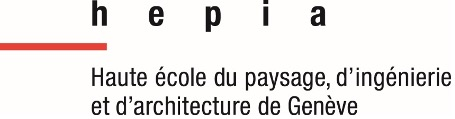
\includegraphics[height=1.29cm]{template/images/title/hepia_logo}};
	\tikz[remember picture,overlay] \node[shift={(-4.238cm,-1.97cm)}]
	at (current page.north east)
	{
\includegraphics[height=1.29cm]{template/images/title/hes-so_geneve_logo}};

\addcontentsline{toc}{chapter}{Résumé} % Adding toc entry
\thispagestyle{noheader}

\begin{spacing}{0.956}
\vspace{0.5cm}

La lumière Cherenkov est un phénomène physique similaire à un boom supersonique dans le domaine électromagnétique.
Lorsque des particules chargées entrent dans notre atmosphère à la vitesse de la lumière, 
elles entament une réaction en chaîne qui produit une pluie de lumière atmosphérique.
L’observation de ces pluies nous permet de mieux comprendre les mécanismes de la physique des particules. 
Dans cette optique, l’UNIGE travaille sur la mission pionnière du télescope spatial Terzina. 
Ce télescope a pour but de détecter et d’étudier les neutrinos de manière indirecte en observant les pluies de lumière atmosphérique
produites par ceux-ci à partir de leur interaction avec le limbe de la Terre. Lors de sa conception, il s'est avéré 
que le télescope recueillera plus de données qu'il sera capable de transmettre au sol.
Le but initial de ce projet consistait à créer un modèle de réseau de neurones embarquable à bord du satellite,
afin de réduire l'utilisation de la bande passante; pour cela, le réseau neuronal effectuera une analyse des données des capteurs
afin de détecter la quantité de photons provenant d'une pluie atmosphérique afin d'aider à cibler des événements scientifiquement plus importants.  
Suite à des délais de production de certains composants essentiels au fonctionnement du réseau neuronal à bord du satellite,
le projet a été adapté pour des télescopes au sol. Ceux-ci rencontrent des problèmes similaires de haute utilisation 
de stockage et de ressources de calcul à cause de la quantité astronomique de données recueillies.
Un réseau de neurones similaire pourrait donc leur être utile.
Lors de ce travail, j'ai commencé par étudier le phénomène physique et le fonctionnement des capteurs. 
J'ai ensuite pris en main les différents simulateurs de données. 
Avec ces données, j'ai testé différentes architectures de réseau neuronaux pour trouver un modèle performant.

\vfill
\begin{center}
	{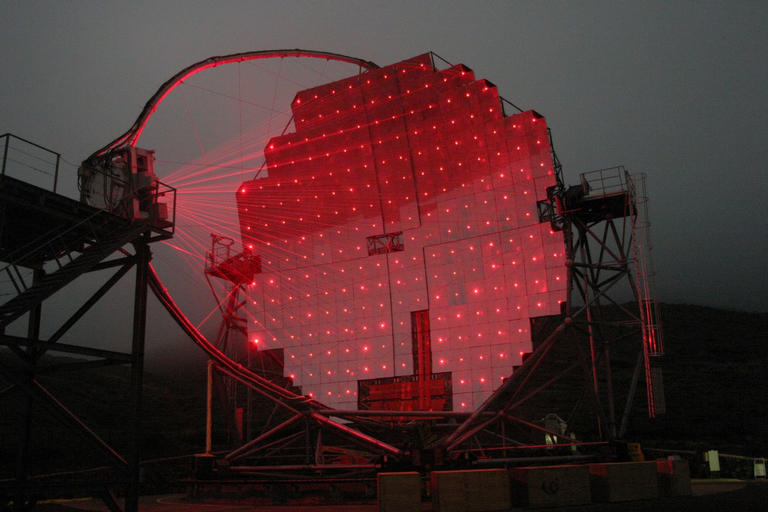
\includegraphics[width=0.4\linewidth]{MagicCalibration.jpg}}\\*
\vfill
%% CONTENT ENDS HERE

{
%%%%%%%%%%%%%%%%%%%%%%%%%%%%%%%%%%%%%%%%%%%%%%%%%%%%%%%%%%%%%%%%%%%%%%%%%%%%%%%%
%%%%%%%%%%%%%%%%%%%%%%%%%% DO NOT MODIFY THE TABLE BELOW %%%%%%%%%%%%%%%%%%%%%%%
%%%%%%%%%%%%%%%%%%%%%%%%%%%%%%%%%%%%%%%%%%%%%%%%%%%%%%%%%%%%%%%%%%%%%%%%%%%%%%%%
	\begin{tabular*}{16cm}{p{7.59cm} p{7.58cm}}
		\small Candidat-e:					&	\small Professeur-e(s) responsable(s):\\*[10pt]
		\small\textbf{\textsc{\Author}}		&	\small\textbf{\textsc{\Professor}}\\*[10pt]
		\footnotesize  Filière d’études : ISC	&	\footnotesize  \textbf{En collaboration avec:} UNIGE\\*[10pt]
		\footnotesize  {} & \footnotesize  Travail de bachelor soumis à une convention de stage en entreprise: \Convention\\*[20pt]
		\footnotesize  {} & \footnotesize  Travail soumis à un contrat de confidentialité: \Confidentiel\\*[10pt]
	\end{tabular*}\\*[1.9cm]
}
\end{center}
\end{spacing}
